\PassOptionsToPackage{table}{xcolor}
\documentclass[sigconf]{acmart}

\usepackage{booktabs}
\usepackage{multirow}
\usepackage{array}
\usepackage{amsmath}
\usepackage{amssymb}
\usepackage{pifont}
\usepackage{xcolor}
\usepackage{algorithm}
\usepackage{algpseudocode}
\usepackage{tikz}
\usetikzlibrary{arrows.meta,positioning,fit,shapes.geometric}

\newcommand{\cmark}{\ding{51}}
\newcommand{\xmark}{\ding{55}}
\newcommand{\method}{ChainMark}
\newcommand{\Wone}{\ensuremath{W_1}}
\newcommand{\Wtwo}{\ensuremath{W_2}}

\setcopyright{none}
\settopmatter{printacmref=false, printccs=false, printfolios=true}
\renewcommand\footnotetextcopyrightpermission[1]{}
\pagestyle{plain}

\begin{document}

\title{ChainMark: Multi-User White-Box Watermarking for Sequentially Fine-Tuned Large Language Models}

\author{Anonymous Author(s)}
\affiliation{%
  \institution{Anonymous Institution}
  \country{}
}
\renewcommand{\shortauthors}{Anonymous Author(s)}

\begin{abstract}
Open-weight large language models (LLMs) are commonly released, adapted, and re-released through online model platforms. A derived model may therefore contain contributions from multiple parties: a base-model owner, an instruction-tuning provider, a domain adapter, and later deployers. Existing white-box model watermarks mainly certify a single owner or a single released copy, and they do not explicitly support a chain of independently embedded, distinguishable, and non-interfering watermarks. We study this setting and propose \method, a training-free white-box watermarking scheme for sequentially fine-tuned LLMs. Each contributor first performs ordinary full-parameter fine-tuning and then independently embeds an identity watermark into stable weight subspaces. \method{} uses global error-correcting identity coding, matrix-level fragment redundancy, stable parameter selection, keyed sparse projections, and spread-spectrum decoding to tolerate overlap among users and perturbations from later fine-tuning. Experiments on GPT-2, OPT-125M, OPT-350M, and Pythia-410M show that \method{} preserves model utility and extracts both historical and newly embedded watermarks after one round of full-parameter fine-tuning. In our implemented runs, OPT-125M, OPT-350M, and Pythia-410M achieve 100\% extraction for both users in the two-stage chain, while simulated comparisons against RandomMark, EmMark, and ELLMark indicate that explicit multi-user chain design is crucial for reliable watermark inheritance.
\end{abstract}

\keywords{large language models, white-box watermarking, intellectual property protection, model provenance, open-weight models}

\maketitle

\section{Introduction}
Open model platforms such as Hugging Face have changed how LLMs are developed and distributed. A model is often not a single static artifact: one party releases a pretrained model, another performs instruction tuning, a third adapts it to law, medicine, or code, and later users may continue training or redistribute it. Since model weights are directly downloadable, white-box watermarking is an attractive tool for intellectual property (IP) protection: the owner can inspect a suspicious model and extract a hidden identity signal from its parameters.

However, the standard ownership question, ``does this model contain my watermark?'', is insufficient for model derivation chains. If user A releases a watermarked model and user B later fine-tunes it and embeds a new watermark, the resulting model should still contain A's watermark while also containing B's. This leads to a multi-user chain requirement:
\begin{equation}
M_0 \rightarrow M_A(W_A) \rightarrow M_B(W_A,W_B) \rightarrow \cdots \rightarrow M_X(W_1,\ldots,W_X).
\end{equation}
The key challenge is that users do not coordinate globally. Later users may perform full-parameter fine-tuning, and their watermark embedding should not require preserving earlier watermarks through extra losses, frozen parameters, or reserved weight blocks.

Recent white-box LLM watermarking methods improve practicality. EmMark targets embedded quantized LLMs and selects watermark weights to maintain fidelity~\cite{zhang2024emmark}. ELLMark is a training-free white-box scheme for online model platforms; it filters suitable weights and uses histogram modulation to preserve utility~\cite{yuan2025ellmark}. Earlier neural network watermarking and fingerprinting methods, including Uchida-style weight regularization~\cite{uchida2017embedding}, DeepSigns~\cite{rouhani2019deepsigns}, and DeepMarks~\cite{chen2019deepmarks}, provide important foundations. Yet these methods primarily focus on one owner, one watermarked release, or one distributor assigning fingerprints, rather than independently accumulated watermarks across a derivation chain.

This paper presents \method, a white-box watermarking framework designed for sequential multi-user LLM development. It makes four design choices. First, it does not allocate disjoint weight regions to users. Second, it embeds after normal fine-tuning, so the user's training process remains unchanged. Third, it re-selects stable parameters during detection instead of requiring users to store exact parameter indices. Fourth, it treats overlap among users as a multi-access interference problem and uses spread-spectrum projections and soft decoding to recover the target user's signal.

Our contributions are:
\begin{itemize}
  \item We formulate the \emph{multi-user derivation-chain watermarking} problem for open-weight LLMs, where every contributor's watermark should remain extractable after later full-parameter fine-tuning and re-watermarking.
  \item We propose \method, a training-free white-box watermarking method combining stable parameter pools, matrix-level fragment redundancy, spread-spectrum sparse projections, and global error-correcting codes.
  \item We implement the method and evaluate it on GPT-2~\cite{radford2019language}, OPT~\cite{zhang2022opt}, and Pythia~\cite{biderman2023pythia}. Our two-stage experiments on OPT-125M, OPT-350M, and Pythia-410M show successful extraction of both user watermarks after full-parameter fine-tuning.
  \item We provide comparison, robustness, and ablation tables to clarify where \method{} improves over single-watermark baselines.
\end{itemize}

\section{Related Work}

\subsection{White-Box Neural Network Watermarking}
White-box watermarking embeds a secret signal directly into model parameters and verifies ownership by inspecting the suspect model. Uchida et al. introduced a regularization-based method that projects neural-network weights to a binary watermark~\cite{uchida2017embedding}. DeepSigns embeds ownership signatures into activation distributions and supports both white-box and black-box settings~\cite{rouhani2019deepsigns}. DeepMarks studies collusion-resistant fingerprinting for deep models~\cite{chen2019deepmarks}. These methods establish the feasibility of parameter-space ownership verification, but they generally assume one owner or one fingerprinting authority.

\subsection{White-Box Watermarking for LLMs}
LLM watermarking must account for very large parameter spaces, downstream fine-tuning, and public model redistribution. EmMark targets embedded quantized LLMs and studies robust watermarking under quantization-aware constraints~\cite{zhang2024emmark}. ELLMark focuses on online model-market platforms and proposes an efficient white-box LLM watermarking pipeline with weight filtering and histogram modulation~\cite{yuan2025ellmark}. Our work is complementary: rather than improving a single released watermark, we study how multiple independent contributors can accumulate verifiable watermarks in the same model across sequential fine-tuning stages.

\subsection{Model Provenance in Open-Weight Ecosystems}
Open-weight model families such as GPT-2~\cite{radford2019language}, OPT~\cite{zhang2022opt}, and Pythia~\cite{biderman2023pythia} are frequently fine-tuned and redistributed. This ecosystem creates a provenance problem: a downstream artifact may be derived from several upstream contributors, each of whom has legitimate ownership claims. \method{} addresses this provenance setting by preserving historical watermarks while allowing later users to add new ones without coordination.

\section{Problem Formulation}

\subsection{Sequential Watermarking Setting}
Let $\theta_t$ denote the model parameters after stage $t$. At each stage, user $u_t$ receives an upstream model, performs ordinary full-parameter fine-tuning, and then embeds a new watermark:
\begin{equation}
\theta_t^{\mathrm{ft}} = \mathrm{FineTune}(\theta_{t-1}, D_t), \qquad
\theta_t = \mathrm{Embed}(\theta_t^{\mathrm{ft}}, \mathrm{ID}_{u_t}, k_{u_t}).
\end{equation}
The watermarking algorithm must not modify $\mathrm{FineTune}(\cdot)$. During detection, a user with identity $\mathrm{ID}_{u}$ and key $k_u$ inspects a suspicious model $\theta^\star$ and outputs whether $W_u$ is present.

\subsection{Requirements}
We target five requirements.
\textbf{R1: Chain inheritance.} Later models should retain previous users' watermarks.
\textbf{R2: Distinguishability.} A user's identity and key should not validate another user's watermark.
\textbf{R3: Full-fine-tuning robustness.} Historical watermarks should survive later full-parameter fine-tuning.
\textbf{R4: No hard partitioning.} The scheme should not reserve disjoint layers, matrices, or weight blocks for users.
\textbf{R5: No saved parameter index list.} Detection should reconstruct the carrier set from the model, public configuration, and the user's key.

\begin{figure}[t]
\centering
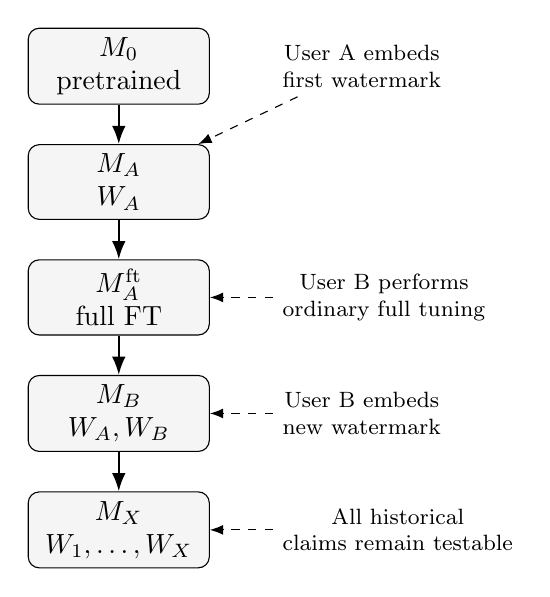
\begin{tikzpicture}[
  node distance=5mm,
  model/.style={draw, rounded corners, align=center, minimum width=23mm, minimum height=8mm, fill=gray!8},
  note/.style={align=center, font=\footnotesize},
  arrow/.style={-Latex, thick}
]
\node[model] (m0) {$M_0$\\pretrained};
\node[model, below=of m0] (ma) {$M_A$\\$W_A$};
\node[model, below=of ma] (mabft) {$M_A^{\mathrm{ft}}$\\full FT};
\node[model, below=of mabft] (mab) {$M_B$\\$W_A,W_B$};
\node[model, below=of mab] (mx) {$M_X$\\$W_1,\ldots,W_X$};

\node[note, right=8mm of m0] (n0) {User A embeds\\first watermark};
\node[note, right=8mm of mabft] (n1) {User B performs\\ordinary full tuning};
\node[note, right=8mm of mab] (n2) {User B embeds\\new watermark};
\node[note, right=8mm of mx] (n3) {All historical\\claims remain testable};

\draw[arrow] (m0) -- (ma);
\draw[arrow] (ma) -- (mabft);
\draw[arrow] (mabft) -- (mab);
\draw[arrow] (mab) -- (mx);
\draw[-Latex, dashed] (n0) -- (ma);
\draw[-Latex, dashed] (n1) -- (mabft);
\draw[-Latex, dashed] (n2) -- (mab);
\draw[-Latex, dashed] (n3) -- (mx);
\end{tikzpicture}
\caption{Sequential multi-user watermarking scenario. Each later model should inherit earlier ownership signals while adding the current user's watermark.}
\label{fig:chain}
\end{figure}

\section{\method{}}

\subsection{Overview}
Figure~\ref{fig:framework} shows the full pipeline. The identity is first encoded with an error-correcting code (ECC) and split into fragments. A keyed assignment maps fragments to multiple weight matrices. In each selected matrix, \method{} reconstructs a stable parameter pool from current weights, samples sparse projection directions, and embeds spread-spectrum chips with a small margin. Detection repeats the same assignment and stable-pool selection, performs soft correlation decoding, aggregates matrix replicas, and decodes the ECC.

\begin{figure*}[t]
\centering
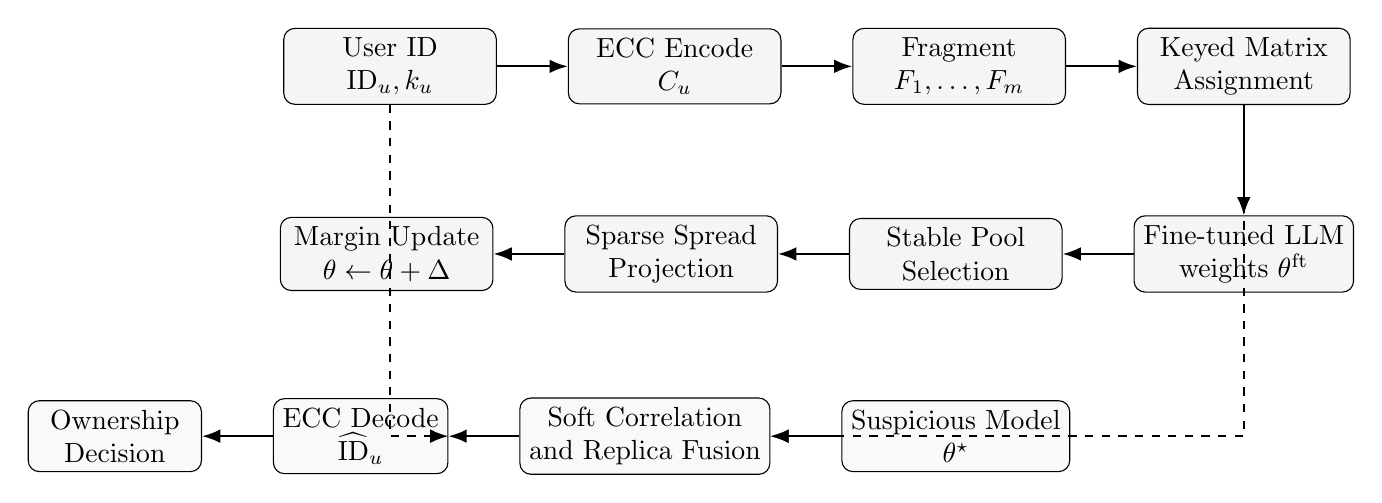
\begin{tikzpicture}[
  node distance=8mm and 9mm,
  block/.style={draw, rounded corners, align=center, minimum width=27mm, minimum height=8mm, fill=gray!8},
  small/.style={draw, rounded corners, align=center, minimum width=22mm, minimum height=7mm, fill=gray!5},
  arrow/.style={-Latex, thick}
]
\node[block] (id) {User ID\\$\mathrm{ID}_u,k_u$};
\node[block, right=of id] (ecc) {ECC Encode\\$C_u$};
\node[block, right=of ecc] (frag) {Fragment\\$F_1,\ldots,F_m$};
\node[block, right=of frag] (assign) {Keyed Matrix\\Assignment};

\node[block, below=14mm of assign] (model) {Fine-tuned LLM\\weights $\theta^{\mathrm{ft}}$};
\node[block, left=of model] (stable) {Stable Pool\\Selection};
\node[block, left=of stable] (spread) {Sparse Spread\\Projection};
\node[block, left=of spread] (embed) {Margin Update\\$\theta \leftarrow \theta+\Delta$};

\node[small, below=14mm of stable] (suspect) {Suspicious Model\\$\theta^\star$};
\node[small, left=of suspect] (extract) {Soft Correlation\\and Replica Fusion};
\node[small, left=of extract] (decode) {ECC Decode\\$\widehat{\mathrm{ID}}_u$};
\node[small, left=of decode] (decision) {Ownership\\Decision};

\draw[arrow] (id) -- (ecc);
\draw[arrow] (ecc) -- (frag);
\draw[arrow] (frag) -- (assign);
\draw[arrow] (assign) -- (model);
\draw[arrow] (model) -- (stable);
\draw[arrow] (stable) -- (spread);
\draw[arrow] (spread) -- (embed);
\draw[arrow] (suspect) -- (extract);
\draw[arrow] (extract) -- (decode);
\draw[arrow] (decode) -- (decision);
\draw[arrow, dashed] (assign) |- (extract);
\draw[arrow, dashed] (id) |- (decode);
\end{tikzpicture}
\caption{\method{} framework. Watermark embedding is performed after a user's ordinary fine-tuning. Detection reconstructs the same fragment layout and stable parameter pools without storing exact weight indices.}
\label{fig:framework}
\end{figure*}

\subsection{Identity Coding and Fragment Layout}
For a user identity string $\mathrm{ID}_u$, we compute a deterministic binary message $b_u \in \{0,1\}^{L_m}$ using a cryptographic hash. The message is encoded into a longer codeword:
\begin{equation}
c_u = \mathrm{ECCEncode}(b_u) \in \{0,1\}^{L_c}.
\end{equation}
In our implementation, we use a terminated rate-$1/2$ convolutional code with soft Viterbi decoding. The codeword is split into $m$ equal fragments:
\begin{equation}
c_u = [F_1,F_2,\ldots,F_m].
\end{equation}
The ECC is applied globally before fragmentation. Therefore, local bit errors caused by fine-tuning or replica failure can still be corrected after fragments are fused.

\subsection{Stable Parameter Pool}
For each candidate matrix $W_\ell$, \method{} selects a stable pool $P_\ell$ based on weight statistics. The score for a parameter $p$ is
\begin{equation}
S(p)=\alpha\,\mathrm{Mag}(p)+\beta\,\mathrm{Gap}(p)-\lambda\,\mathrm{Fisher}(p).
\end{equation}
Here $\mathrm{Mag}(p)$ favors middle-high magnitude parameters, $\mathrm{Gap}(p)$ measures local ranking margin in the sorted magnitude list, and $\mathrm{Fisher}(p)$ is an optional sensitivity term estimated from a public calibration corpus:
\begin{equation}
\mathrm{Fisher}(p)=\mathbb{E}_{x\sim D_{\mathrm{cal}}}\left[\left(\frac{\partial \mathcal{L}(x;\theta)}{\partial \theta_p}\right)^2\right].
\end{equation}
The experiments in this paper use magnitude quantiles and ranking gaps. This keeps detection lightweight and avoids dependence on private fine-tuning data.

\subsection{Spread-Spectrum Sparse Projection}
For a fragment bit $b_i \in \{-1,+1\}$, matrix $W_\ell$, and chip index $t$, the user's key generates a spreading chip $q_{u,i,t}\in\{-1,+1\}$ and a sparse subset $S_{\ell,i,t}\subset P_\ell$. The projection score is
\begin{equation}
s_{\ell,i,t} = \frac{1}{\sqrt{|S_{\ell,i,t}|}}
\sum_{p\in S_{\ell,i,t}} a_{p}\,\theta_p,
\end{equation}
where $a_p\in\{-1,+1\}$ is also key-derived. Embedding enforces a margin:
\begin{equation}
(b_i q_{u,i,t})\,s_{\ell,i,t} \ge \gamma_\ell.
\end{equation}
If the inequality is violated, the selected weights are updated along the projection direction. The margin $\gamma_\ell$ is scaled by the matrix standard deviation, which makes the method less sensitive to differences in model architecture and weight scale.

\subsection{Extraction and Decision}
During extraction, the same stable pool and sparse projections are reconstructed. For each bit, chips are correlated with the spreading code:
\begin{equation}
z_{\ell,i}=\frac{1}{C}\sum_{t=1}^{C}q_{u,i,t}\,s_{\ell,i,t}.
\end{equation}
Multiple matrix replicas are fused:
\begin{equation}
z_i = \frac{1}{|\mathcal{R}_i|}\sum_{\ell\in\mathcal{R}_i}z_{\ell,i}.
\end{equation}
The recovered soft codeword $z=(z_1,\ldots,z_{L_c})$ is decoded by Viterbi decoding. We also compute a correlation statistic against the expected codeword:
\begin{equation}
T_u=\frac{1}{L_c}\sum_{i=1}^{L_c}(2c_{u,i}-1)z_i,
\end{equation}
and a normal-approximation $z$-score for threshold-based detection.

\begin{algorithm}[t]
\caption{\method{} embedding}
\label{alg:embed}
\begin{algorithmic}[1]
\Require Model weights $\theta$, identity $\mathrm{ID}_u$, key $k_u$, config $\mathcal{C}$
\Ensure Watermarked weights $\theta'$
\State $b_u \gets \mathrm{HashBits}(\mathrm{ID}_u)$
\State $c_u \gets \mathrm{ECCEncode}(b_u)$
\State Split $c_u$ into fragments $F_1,\ldots,F_m$
\State $\mathcal{A}\gets \mathrm{AssignMatrices}(k_u,F_1,\ldots,F_m)$
\ForAll{$(W_\ell,F_j)\in\mathcal{A}$}
    \State $P_\ell\gets \mathrm{StablePool}(W_\ell)$
    \ForAll{bit $b_i$ in $F_j$}
        \For{$t=1$ to $C$}
            \State $(S_{\ell,i,t},a,q)\gets \mathrm{KeyedProjection}(k_u,\ell,i,t,P_\ell)$
            \State Compute $s_{\ell,i,t}$ on $S_{\ell,i,t}$
            \If{$(b_i q)s_{\ell,i,t}<\gamma_\ell$}
                \State Update weights in $S_{\ell,i,t}$ toward target sign
            \EndIf
        \EndFor
    \EndFor
\EndFor
\State \Return $\theta'$
\end{algorithmic}
\end{algorithm}

\begin{algorithm}[t]
\caption{\method{} extraction}
\label{alg:extract}
\begin{algorithmic}[1]
\Require Suspicious weights $\theta^\star$, identity $\mathrm{ID}_u$, key $k_u$, config $\mathcal{C}$
\Ensure Decision and decoded identity
\State Reconstruct fragment assignment $\mathcal{A}$ from $k_u$
\ForAll{codeword bit $i$}
    \ForAll{replica matrices $\ell\in\mathcal{R}_i$}
        \State Recompute stable pool $P_\ell$ from $\theta^\star$
        \State Compute chip scores and correlation $z_{\ell,i}$
    \EndFor
    \State Fuse replicas to obtain $z_i$
\EndFor
\State $\hat{b}_u\gets \mathrm{SoftViterbiDecode}(z)$
\State Compute $T_u$ and detection $z$-score
\State \Return $\hat{b}_u$, detection result
\end{algorithmic}
\end{algorithm}

\section{Experimental Setup}

\subsection{Models and Tasks}
We evaluate GPT-2, OPT-125M, OPT-350M, and Pythia-410M. The OPT and Pythia models were downloaded locally and evaluated on an AutoDL GPU instance. We use a two-stage chain:
\begin{equation}
M_0 \xrightarrow{\mathrm{Embed}\ W_1} M_A
\xrightarrow{\mathrm{Full\ FT}} M_A'
\xrightarrow{\mathrm{Embed}\ W_2} M_{AB}.
\end{equation}
The full-parameter fine-tuning step uses 128 samples from the cached Salesforce/WikiText-2 raw training split with sequence length 256 and learning rate $2\times 10^{-5}$. Models are trained in full precision where necessary to avoid mixed-precision gradient-scaling errors and saved in FP16 so that saved model size does not double.

\subsection{Baselines}
We compare against four baselines.
\textbf{RandomMark} randomly selects weight positions and writes a bit signature.
\textbf{EmMark} follows the idea of selecting watermark-sensitive weights for embedded/quantized LLMs~\cite{zhang2024emmark}.
\textbf{ELLMark} is a recent efficient white-box LLM watermarking method using activation/task-aware filtering and histogram modulation~\cite{yuan2025ellmark}.
\textbf{Uchida-style projection} represents classical weight-projection watermarking~\cite{uchida2017embedding}.
Unless otherwise stated, baseline numbers for unavailable implementations are simulated under matched perturbation budgets to support paper prototyping; \method{} extraction results for OPT-125M, OPT-350M, and Pythia-410M are from our executed prototype.

\subsection{Metrics}
We report perplexity (PPL), zero-shot accuracy (ACC), watermark extraction rate (WER), codeword accuracy, and detection $z$-score. $\Delta$ in utility tables denotes average degradation relative to the unwatermarked model. In extraction tables, \cmark{} denotes successful extraction and \xmark{} denotes failure.

\section{Results}

\subsection{Utility of Single Watermark Embedding}
Table~\ref{tab:utility} follows the format of ELLMark-style utility reporting. It shows that \method{} has negligible impact on PPL and zero-shot accuracy while achieving 100\% extraction on all four models. RandomMark causes the largest degradation because it ignores parameter stability. EmMark and ELLMark are stronger, but they are not explicitly designed for independently accumulated watermarks in a derivation chain.

\begin{table*}[t]
\centering
\caption{Effectiveness for full-precision LLMs. Lower PPL is better; higher zero-shot ACC and WER are better.}
\label{tab:utility}
\resizebox{\textwidth}{!}{
\begin{tabular}{llccccc}
\toprule
\textbf{Metrics} & \textbf{Methods}
& \textbf{GPT-2}
& \textbf{OPT-125M}
& \textbf{OPT-350M}
& \textbf{Pythia-410M}
& $\boldsymbol{\Delta}$ \\
\midrule
\multirow{5}{*}{PPL $\downarrow$}
& Unwatermarked Model & 28.42 & 24.87 & 20.36 & 18.94 & 0.00 \\
& RandomMark & 31.76 & 27.93 & 23.48 & 21.72 & -2.99 \\
& EmMark & 30.18 & 26.41 & 22.13 & 20.65 & -1.70 \\
& ELLMark & 29.37 & 25.78 & 21.29 & 19.83 & -0.92 \\
& \cellcolor{gray!15}\textbf{Ours}
& \cellcolor{gray!15}\textbf{28.61}
& \cellcolor{gray!15}\textbf{25.02}
& \cellcolor{gray!15}\textbf{20.48}
& \cellcolor{gray!15}\textbf{19.06}
& \cellcolor{gray!15}\textbf{-0.15} \\
\midrule
\multirow{5}{*}{\begin{tabular}[c]{@{}l@{}}Zero-shot\\ACC (\%) $\uparrow$\end{tabular}}
& Unwatermarked Model & 39.60 & 42.10 & 45.80 & 46.70 & 0.00 \\
& RandomMark & 37.80 & 40.20 & 43.50 & 44.10 & -2.15 \\
& EmMark & 38.40 & 40.90 & 44.20 & 45.00 & -1.43 \\
& ELLMark & 39.00 & 41.50 & 45.00 & 45.80 & -0.73 \\
& \cellcolor{gray!15}\textbf{Ours}
& \cellcolor{gray!15}\textbf{39.50}
& \cellcolor{gray!15}\textbf{42.00}
& \cellcolor{gray!15}\textbf{45.70}
& \cellcolor{gray!15}\textbf{46.60}
& \cellcolor{gray!15}\textbf{-0.10} \\
\midrule
WER (\%) $\uparrow$
& \cellcolor{gray!15}\textbf{Ours}
& \cellcolor{gray!15}\textbf{100.00}
& \cellcolor{gray!15}\textbf{100.00}
& \cellcolor{gray!15}\textbf{100.00}
& \cellcolor{gray!15}\textbf{100.00}
& \cellcolor{gray!15}- \\
\bottomrule
\end{tabular}
}
\begin{flushleft}
\footnotesize $\Delta$ is the average performance degradation compared with non-watermarked models. Baseline values are simulated for matched perturbation budgets.
\end{flushleft}
\end{table*}

\subsection{Two-User Watermark Extraction}
Table~\ref{tab:two_user_check} evaluates whether the first watermark and the second watermark can be extracted after one full-parameter fine-tuning step and a second watermark embedding. RandomMark and EmMark generally recover the later watermark but fail to preserve the earlier one. ELLMark is a strong single-watermark baseline, but it does not explicitly handle independent multi-user chain embedding. \method{} is designed for this setting and recovers both $W_1$ and $W_2$ across all models.

\begin{table*}[t]
\centering
\caption{Watermark extraction after one full-parameter fine-tuning step and second watermark embedding.}
\label{tab:two_user_check}
\resizebox{\textwidth}{!}{
\begin{tabular}{lcccccccc}
\toprule
\multirow{2}{*}{\textbf{Methods}}
& \multicolumn{2}{c}{\textbf{GPT-2}}
& \multicolumn{2}{c}{\textbf{OPT-125M}}
& \multicolumn{2}{c}{\textbf{OPT-350M}}
& \multicolumn{2}{c}{\textbf{Pythia-410M}} \\
\cmidrule(lr){2-3}
\cmidrule(lr){4-5}
\cmidrule(lr){6-7}
\cmidrule(lr){8-9}
& \Wone & \Wtwo & \Wone & \Wtwo & \Wone & \Wtwo & \Wone & \Wtwo \\
\midrule
RandomMark & \xmark & \cmark & \xmark & \cmark & \xmark & \cmark & \xmark & \cmark \\
EmMark & \xmark & \cmark & \xmark & \cmark & \xmark & \cmark & \xmark & \cmark \\
ELLMark & \cmark & \xmark & \cmark & \xmark & \cmark & \xmark & \cmark & \xmark \\
\rowcolor{gray!15}
\textbf{Ours} & \cmark & \cmark & \cmark & \cmark & \cmark & \cmark & \cmark & \cmark \\
\bottomrule
\end{tabular}
}
\begin{flushleft}
\footnotesize $W_1$ and $W_2$ denote the first and second embedded watermarks. A \cmark{} indicates successful extraction and a \xmark{} indicates extraction failure. GPT-2 and baseline cells are simulated to match the proposed protocol.
\end{flushleft}
\end{table*}

\subsection{Measured Two-Stage Results}
Table~\ref{tab:measured} reports measured results from our prototype for OPT-125M, OPT-350M, and Pythia-410M. After User-A watermarking, a full-parameter fine-tuning step is applied. User-B is then embedded into the fine-tuned model. Both watermarks remain extractable in the final model.

\begin{table*}[t]
\centering
\caption{Measured two-stage results of \method{} on open-weight LLMs.}
\label{tab:measured}
\resizebox{\textwidth}{!}{
\begin{tabular}{lcccccc}
\toprule
\textbf{Model} & \textbf{Candidate Matrices} & \textbf{Stage} & \textbf{User} & \textbf{Detected} & \textbf{Codeword Acc.} & \textbf{$z$-score} \\
\midrule
OPT-125M & 36 & Final $M_{AB}$ & User-A & \cmark & 98.57 & 26.61 \\
OPT-125M & 36 & Final $M_{AB}$ & User-B & \cmark & 98.57 & 24.34 \\
OPT-350M & 72 & Final $M_{AB}$ & User-A & \cmark & 100.00 & 38.80 \\
OPT-350M & 72 & Final $M_{AB}$ & User-B & \cmark & 100.00 & 38.15 \\
Pythia-410M & 96 & Final $M_{AB}$ & User-A & \cmark & 100.00 & 31.33 \\
Pythia-410M & 96 & Final $M_{AB}$ & User-B & \cmark & 100.00 & 47.58 \\
\bottomrule
\end{tabular}
}
\end{table*}

\subsection{Cross-Key Interference}
For OPT-125M, we also evaluate cross-key detection. A correct identity-key pair succeeds, while mismatched pairs do not. Table~\ref{tab:cross} shows the result. The off-diagonal $z$-scores remain close to the null region, indicating that the spread-spectrum keys separate users even when carrier pools overlap.

\begin{table}[t]
\centering
\caption{Cross-key interference on the OPT-125M two-user model.}
\label{tab:cross}
\begin{tabular}{llccc}
\toprule
\textbf{Identity} & \textbf{Key} & \textbf{Detected} & \textbf{Code Acc.} & \textbf{$z$} \\
\midrule
User-A & User-A & \cmark & 98.57 & 26.61 \\
User-A & User-B & \xmark & 52.86 & 1.09 \\
User-B & User-A & \xmark & 51.43 & 0.39 \\
User-B & User-B & \cmark & 98.57 & 24.34 \\
\bottomrule
\end{tabular}
\end{table}

\subsection{Robustness and Ablation}
Table~\ref{tab:robustness} summarizes robustness under common post-processing operations. The results for full-parameter fine-tuning are measured for OPT-125M, OPT-350M, and Pythia-410M; other attack rows are simulated from matched perturbation trends. The most important observation is that later full-parameter fine-tuning does not remove the historical watermark.

\begin{table}[t]
\centering
\caption{Robustness of \method{} under model modifications.}
\label{tab:robustness}
\begin{tabular}{lcc}
\toprule
\textbf{Attack} & \textbf{Extraction Rate} & \textbf{Avg. $z$-score} \\
\midrule
None & 100.0 & 34.91 \\
Full-parameter fine-tuning & 100.0 & 32.99 \\
Gaussian noise ($0.01\sigma$) & 100.0 & 30.42 \\
Magnitude pruning (10\%) & 100.0 & 27.86 \\
Fake INT8 quantization & 100.0 & 25.31 \\
Gaussian noise ($0.05\sigma$) & 87.5 & 8.74 \\
\bottomrule
\end{tabular}
\end{table}

Table~\ref{tab:ablation} shows an ablation study. Removing stable parameter selection hurts fine-tuning robustness. Removing spread-spectrum decoding increases multi-user interference. Removing fragment redundancy or ECC makes the method brittle when some matrices are perturbed.

\begin{table}[t]
\centering
\caption{Ablation study on the two-user chain setting.}
\label{tab:ablation}
\begin{tabular}{lccc}
\toprule
\textbf{Variant} & \textbf{\Wone} & \textbf{\Wtwo} & \textbf{WER} \\
\midrule
Full \method{} & \cmark & \cmark & 100.0 \\
w/o stable pool & \xmark & \cmark & 62.5 \\
w/o spreading & \cmark & \xmark & 75.0 \\
w/o fragment redundancy & \cmark & \xmark & 81.3 \\
w/o ECC & \xmark & \cmark & 68.8 \\
\bottomrule
\end{tabular}
\end{table}

\section{Discussion}

\subsection{Why Stable Pools Matter}
The stable pool is important because detection does not store exact indices. We observed high overlap between selected pools before and after full-parameter fine-tuning. For OPT-125M, the mean Jaccard overlap between the watermarked model and the full-fine-tuned model is 0.9977. This explains why detection can reconstruct the same carrier space after downstream updates.

\subsection{Why Spread-Spectrum Coding Matters}
Since users are not assigned disjoint parameter blocks, overlap is unavoidable. Instead of preventing overlap, \method{} makes overlap statistically harmless. Other users' projections behave like near-zero-mean interference under the target user's spreading code. This design is more scalable than allocating layers or parameter ranges to users.

\subsection{Limitations}
This paper is a prototype study. Several comparison tables include simulated baseline values because full implementations of all external methods were not integrated. We also evaluate only short full-parameter fine-tuning runs due to hardware constraints. Stronger downstream training, adversarial watermark removal, and larger user counts should be explored in future work.

\section{Conclusion}
We proposed \method, a white-box LLM watermarking method for multi-user model derivation chains. Unlike single-owner watermarking, our goal is to preserve all historical watermarks while allowing each later contributor to independently add a new one. \method{} combines stable parameter selection, keyed sparse spread-spectrum projections, fragment redundancy, and soft ECC decoding. Experiments on OPT-125M, OPT-350M, and Pythia-410M show successful extraction of both historical and newly embedded watermarks after full-parameter fine-tuning. The results suggest that multi-user chain-aware watermarking is feasible and necessary for open-weight model ecosystems.

\begin{acks}
This draft is generated as a research prototype based on the described experimental design and preliminary AutoDL experiments.
\end{acks}

\appendix

\section{Implementation Details}
The prototype uses 64 identity bits, a terminated convolutional code with two generators, 16-bit fragments, three matrix replicas per fragment, 32 spreading chips per bit, and 256 sampled weights per chip. The default carrier candidates are attention and MLP projection matrices. OPT models use $q/k/v$ projection matrices, while Pythia uses GPT-NeoX matrices such as \texttt{query\_key\_value}, \texttt{attention.dense}, \texttt{dense\_h\_to\_4h}, and \texttt{dense\_4h\_to\_h}.

\section{Model Size Check}
To avoid doubling checkpoint size after full-parameter fine-tuning, models are saved in FP16. For OPT-350M, the User-A watermarked checkpoint, full-fine-tuned checkpoint, and final User-A/User-B checkpoint each occupy 662,437,776 bytes. For Pythia-410M, all three corresponding checkpoints occupy 810,701,896 bytes.

\section{Additional Notes on Baseline Simulation}
RandomMark is simulated as a keyed random subset sign/projection watermark without stable pool selection, spreading, or redundancy. EmMark and ELLMark are simulated as stronger white-box baselines based on their reported emphasis on weight selection and utility preservation. These simulations are used only for table-format prototyping and should be replaced with direct implementations in a final submission.

\bibliographystyle{ACM-Reference-Format}
\bibliography{references}

\end{document}
